% Schematické překreslení přednášky 3, strany PDF 66; bez číselného měřítka.
\documentclass[border=4mm]{standalone}
\usepackage{fontspec}
\setsansfont{Lato}
\usepackage{amsmath,tikz}
\usetikzlibrary{arrows.meta}
\definecolor{ink}{HTML}{173B4A}
\definecolor{curve}{HTML}{165E96}
\definecolor{pale}{HTML}{EAF1F5}
\definecolor{mark}{HTML}{A52A2A}
\begin{document}
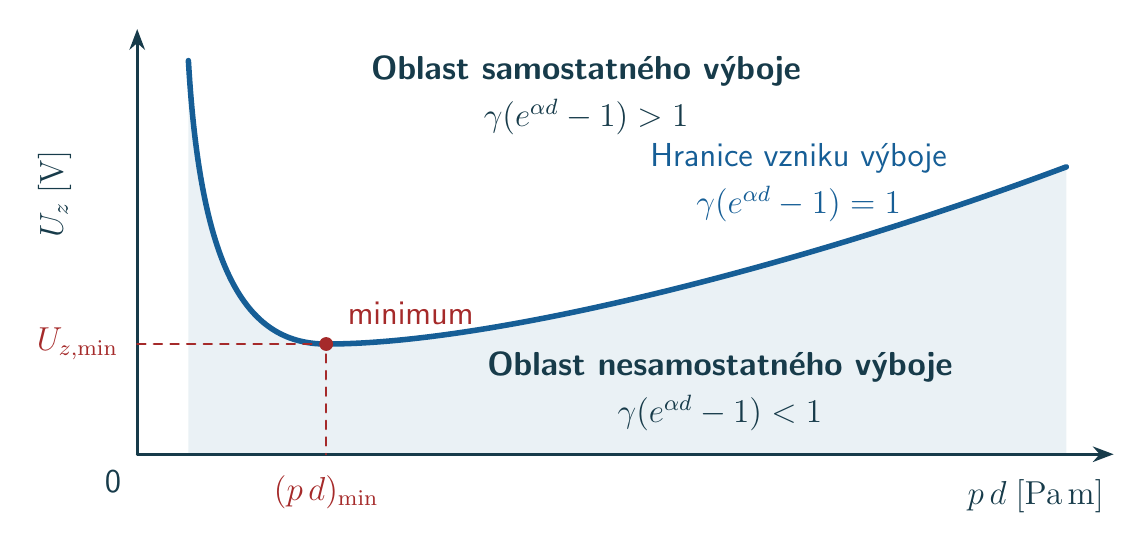
\begin{tikzpicture}[x=1cm,y=1cm,font=\sffamily\fontsize{12}{14}\selectfont,
  >=Stealth,text=ink,line cap=round,line join=round]
  % Tvar odpovídá schématu v přednášce, nejde o fit naměřených dat.
  \path[fill=pale] (.65,5)
    .. controls (.8,2.4) and (1.35,1.4) .. (2.4,1.4)
    .. controls (4.6,1.4) and (8.6,2.45) .. (11.8,3.65)
    -- (11.8,0) -- (.65,0) -- cycle;
  \draw[->,ink,line width=1pt] (0,0) -- (12.4,0);
  \draw[->,ink,line width=1pt] (0,0) -- (0,5.4);
  \node[rotate=90] at (-1.05,3.3) {$U_z\;[\mathrm V]$};
  \node[anchor=north east] at (12.4,-.2) {$p\,d\;[\mathrm{Pa\,m}]$};
  \node[anchor=north east] at (-.08,-.08) {0};
  \draw[curve,line width=2pt] (.65,5)
    .. controls (.8,2.4) and (1.35,1.4) .. (2.4,1.4)
    .. controls (4.6,1.4) and (8.6,2.45) .. (11.8,3.65);
  \draw[draw=mark,dashed,line width=.8pt] (0,1.4) -- (2.4,1.4) -- (2.4,0);
  \fill[fill=mark] (2.4,1.4) circle (2.5pt);
  \node[anchor=east,text=mark] at (-.12,1.4) {$U_{z,\min}$};
  \node[anchor=north,text=mark] at (2.4,-.15) {$(p\,d)_{\min}$};
  \node[anchor=south west,text=mark] at (2.55,1.52) {minimum};
  \node[align=center] at (5.7,4.55)
    {\textbf{Oblast samostatného výboje}\\[3pt]$\gamma(e^{\alpha d}-1)>1$};
  \node[align=center] at (7.4,.8)
    {\textbf{Oblast nesamostatného výboje}\\[3pt]$\gamma(e^{\alpha d}-1)<1$};
  \node[align=center,text=curve] at (8.4,3.45)
    {Hranice vzniku výboje\\[3pt]$\gamma(e^{\alpha d}-1)=1$};
\end{tikzpicture}
\end{document}
